\chapter{Results}

\section{Performance Evaluation}

\section{Ablation Studies}
\label{sec:ablation_studies}

\begin{itemize}
    \item Includes more important initial tests, move less important ones to appendix.
\end{itemize}

\begin{itemize}
    \item GloVe vs random normal distribution. Glove required less tuning since the vector norms already worked well.
\end{itemize}

\section{Hyperparameter Optimisation}

{\color{red}
  \begin{itemize}
    \item wandb \cite{wandb} implementation of bayesian optimisation, using the hyperband early stopping method
  \end{itemize}
}

The effects of the Hyperband method are clearly seen in \figureautorefname{ \ref{fig:hyperparameter_optimisation_validation_loss_and_accuracy}}, where only a few models are trained to completion and less promising models are stopped earlier to encourage exploration of the hyperparameter search space.

\begin{figure}
    \centering
    \begin{subfigure}[t]{\textwidth}
        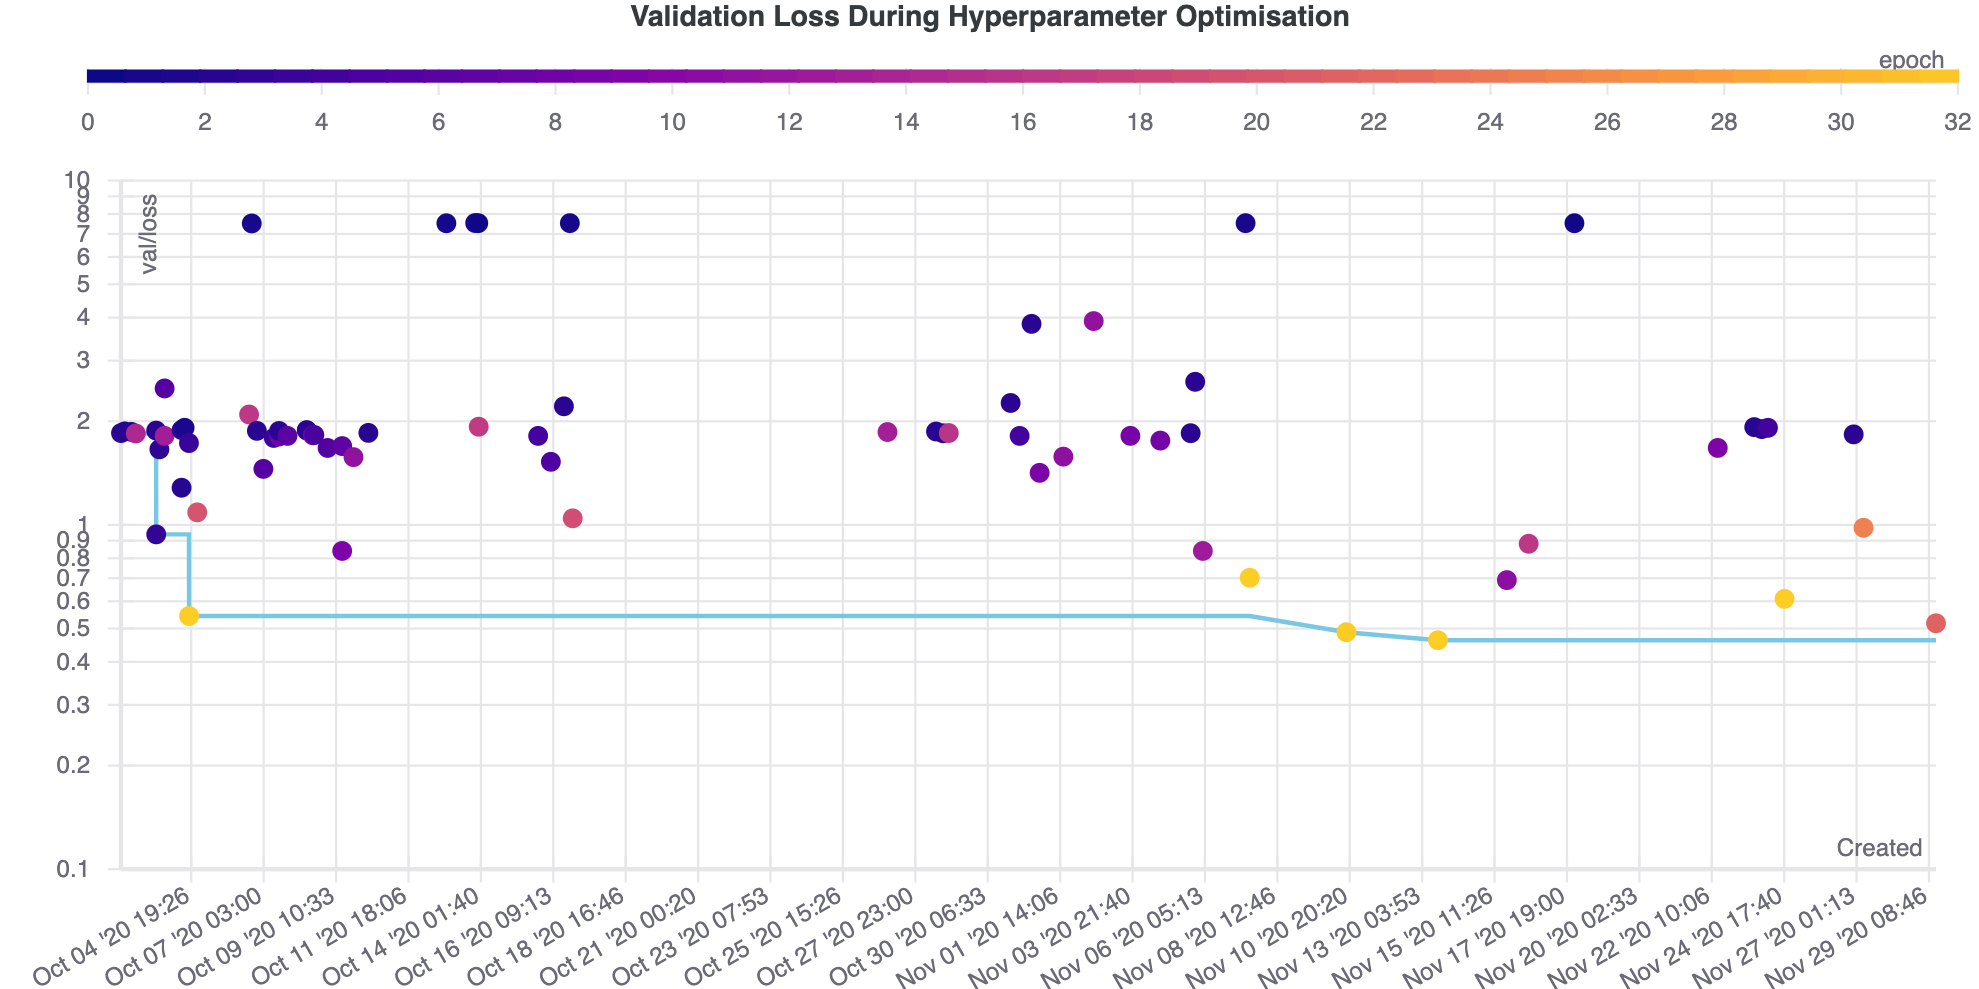
\includegraphics[width=\textwidth]{hyperparameter_optimisation_validation_loss.png}
        \label{fig:hyperparameter_optimisation_validation_loss}
        \caption{Validation loss throughout the hyperparameter optimisation process.}
    \end{subfigure}
    \par\bigskip % force a bit of vertical whitespace
    \par\bigskip
    \begin{subfigure}[b]{\textwidth}
        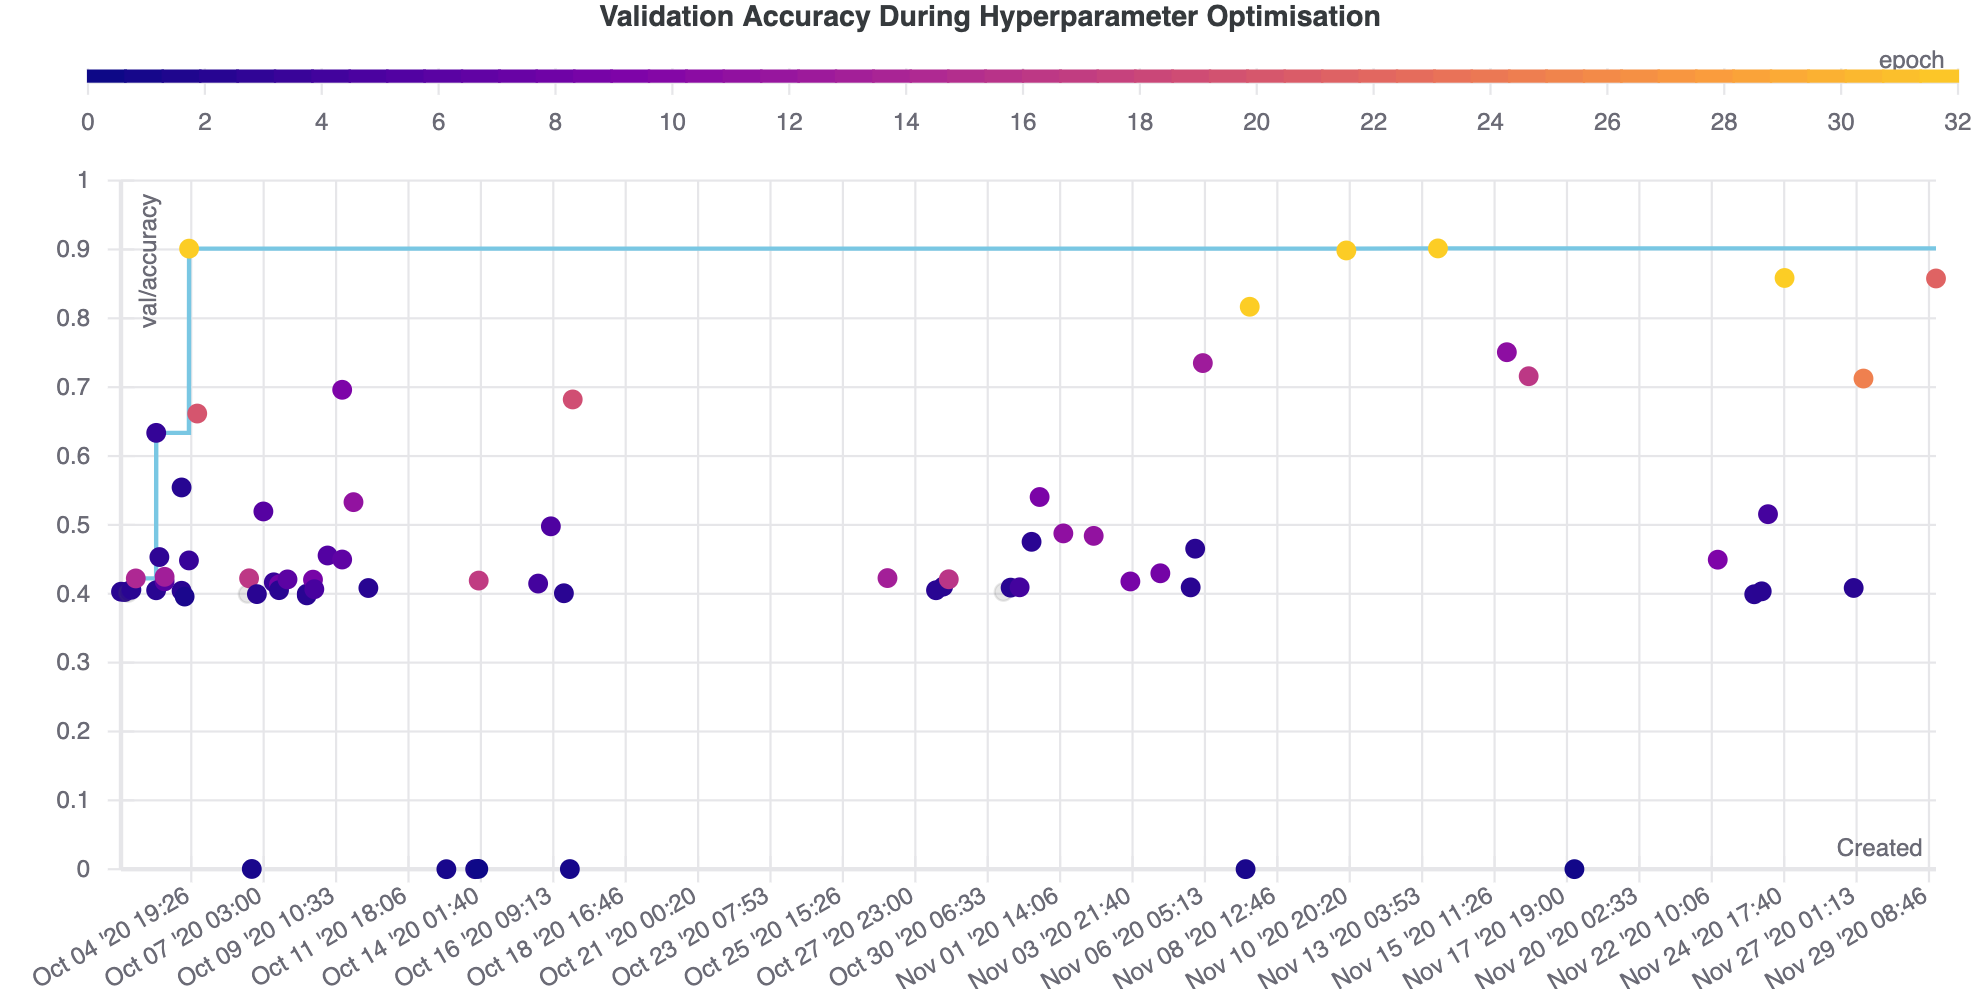
\includegraphics[width=\textwidth]{hyperparameter_optimisation_validation_accuracy.png}
        \label{fig:hyperparameter_optimisation_validation_accuracy}
        \caption{Validation accuracy throughout the hyperparameter optimisation process. Greyed out points correspond to models with a loss greater than 10.}
    \end{subfigure}
    \caption{A summary of validation loss and accuracy throughout the hyperparameter optimisation process. Each point represents a trained model, and its colour indicates how many epochs the model was trained for.}
    \label{fig:hyperparameter_optimisation_validation_loss_and_accuracy}
\end{figure}
 
 
